\documentclass[10pt, oneside]{article} 
\usepackage{amsmath, amsthm, amssymb, calrsfs, wasysym, verbatim, bbm, color, graphicx, geometry}
\usepackage[]{hyperref}
\usepackage{float}
\usepackage{booktabs}
\usepackage{caption}
\usepackage{apacite}
\geometry{tmargin=.75in, bmargin=.25in, lmargin=.75in, rmargin = .75in}  

\newcommand{\R}{\mathbb{R}}
\newcommand{\C}{\mathbb{C}}
\newcommand{\Z}{\mathbb{Z}}
\newcommand{\N}{\mathbb{N}}
\newcommand{\Q}{\mathbb{Q}}
\newcommand{\Cdot}{\boldsymbol{\cdot}}

\newtheorem{thm}{Theorem}
\newtheorem{defn}{Definition}
\newtheorem{conv}{Convention}
\newtheorem{rem}{Remark}
\newtheorem{lem}{Lemma}
\newtheorem{cor}{Corollary}

\newenvironment{problem}[2][Problem]{\begin{trivlist}
    \item[\hskip \labelsep {\bfseries #1}\hskip \labelsep {\bfseries #2.}]}{\end{trivlist}}


\title{Literature Review Assignment: Interdisciplinary Research Methods}
\author{Chirayu Salgarkar}
\date{\today}

\begin{document}

\maketitle

\begin{problem}{$\#1$} 
I am using BibTeX as my citation environment manager. 
\end{problem}

\begin{problem}{$\#2$}
I have set up a Public Google Scholar Account. Here is a screenshot. 
\begin{figure}[H]
    \centering
    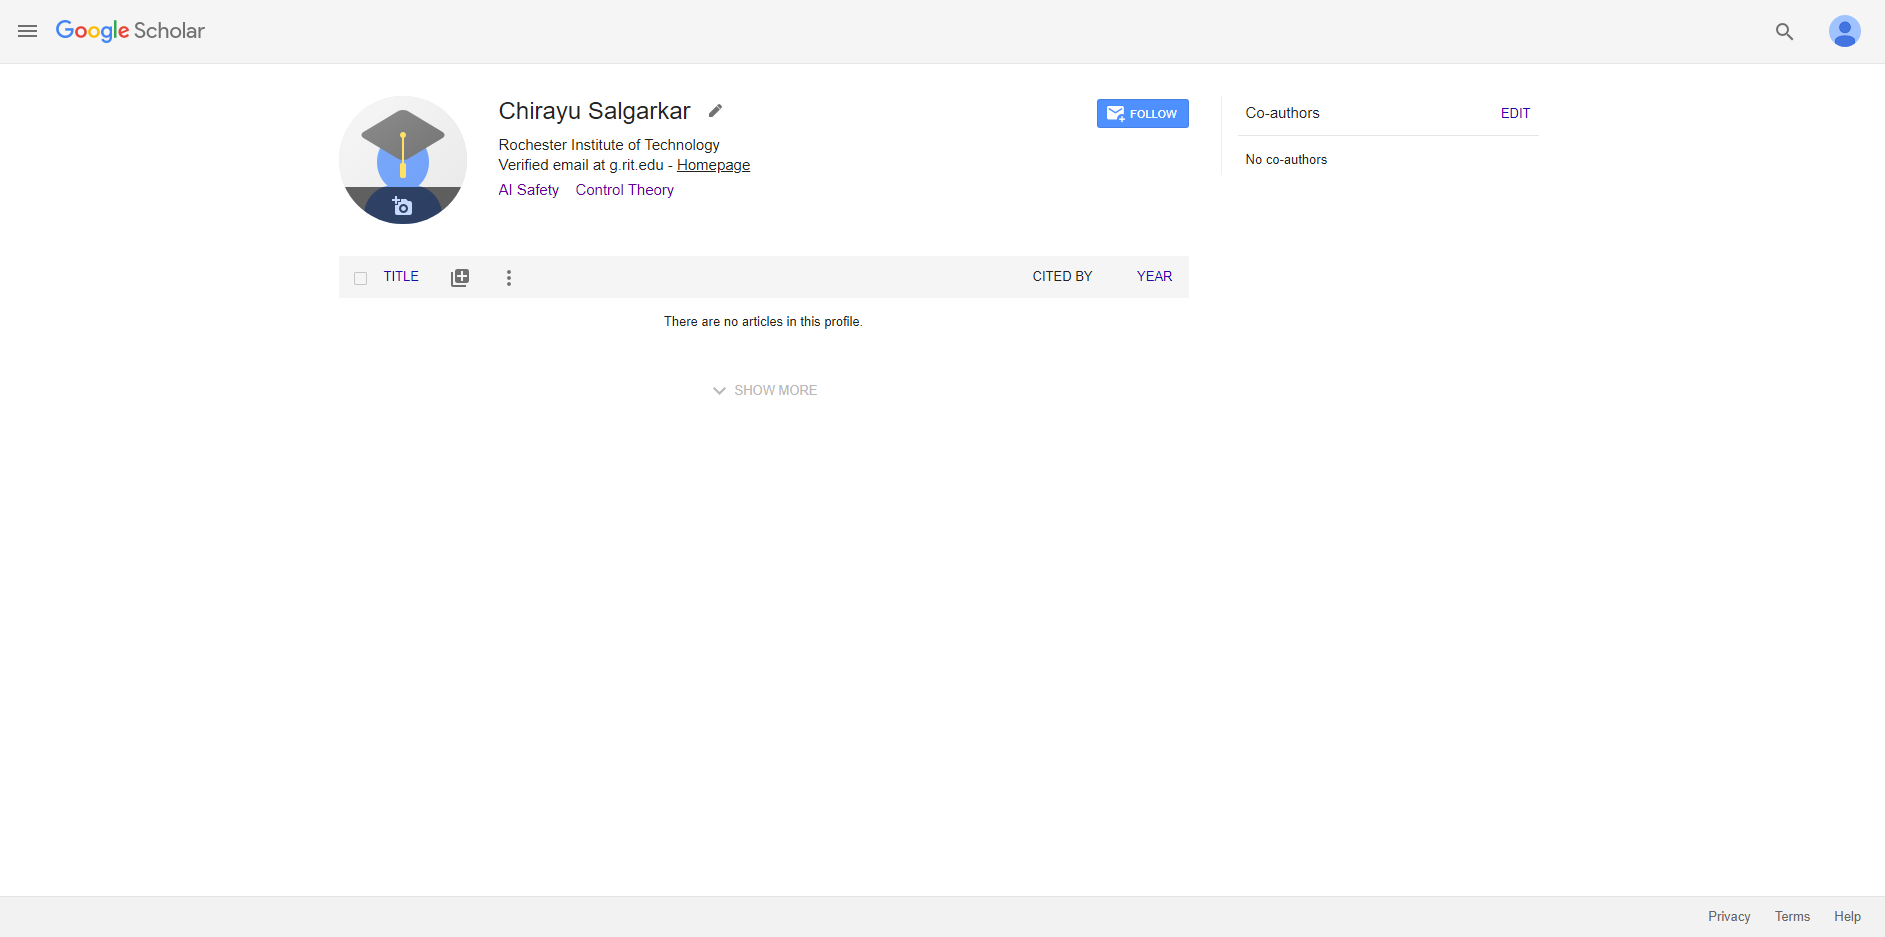
\includegraphics[width = \textwidth]{2024-09-19 18.42.25 scholar.google.com ce7081f53fb7.png}
    \caption{Screenshot of Google Scholar Account. I have set it up as public, but since there are no publications at the outset, searchability is not good.}
    \label{fig:account}
    \end{figure}
\end{problem}


\begin{problem}{$\#2$}
    I have set up Google Scholar Alerts. See Figure \ref{fig:alerts} for details.
        \begin{figure}[H]
        \centering
        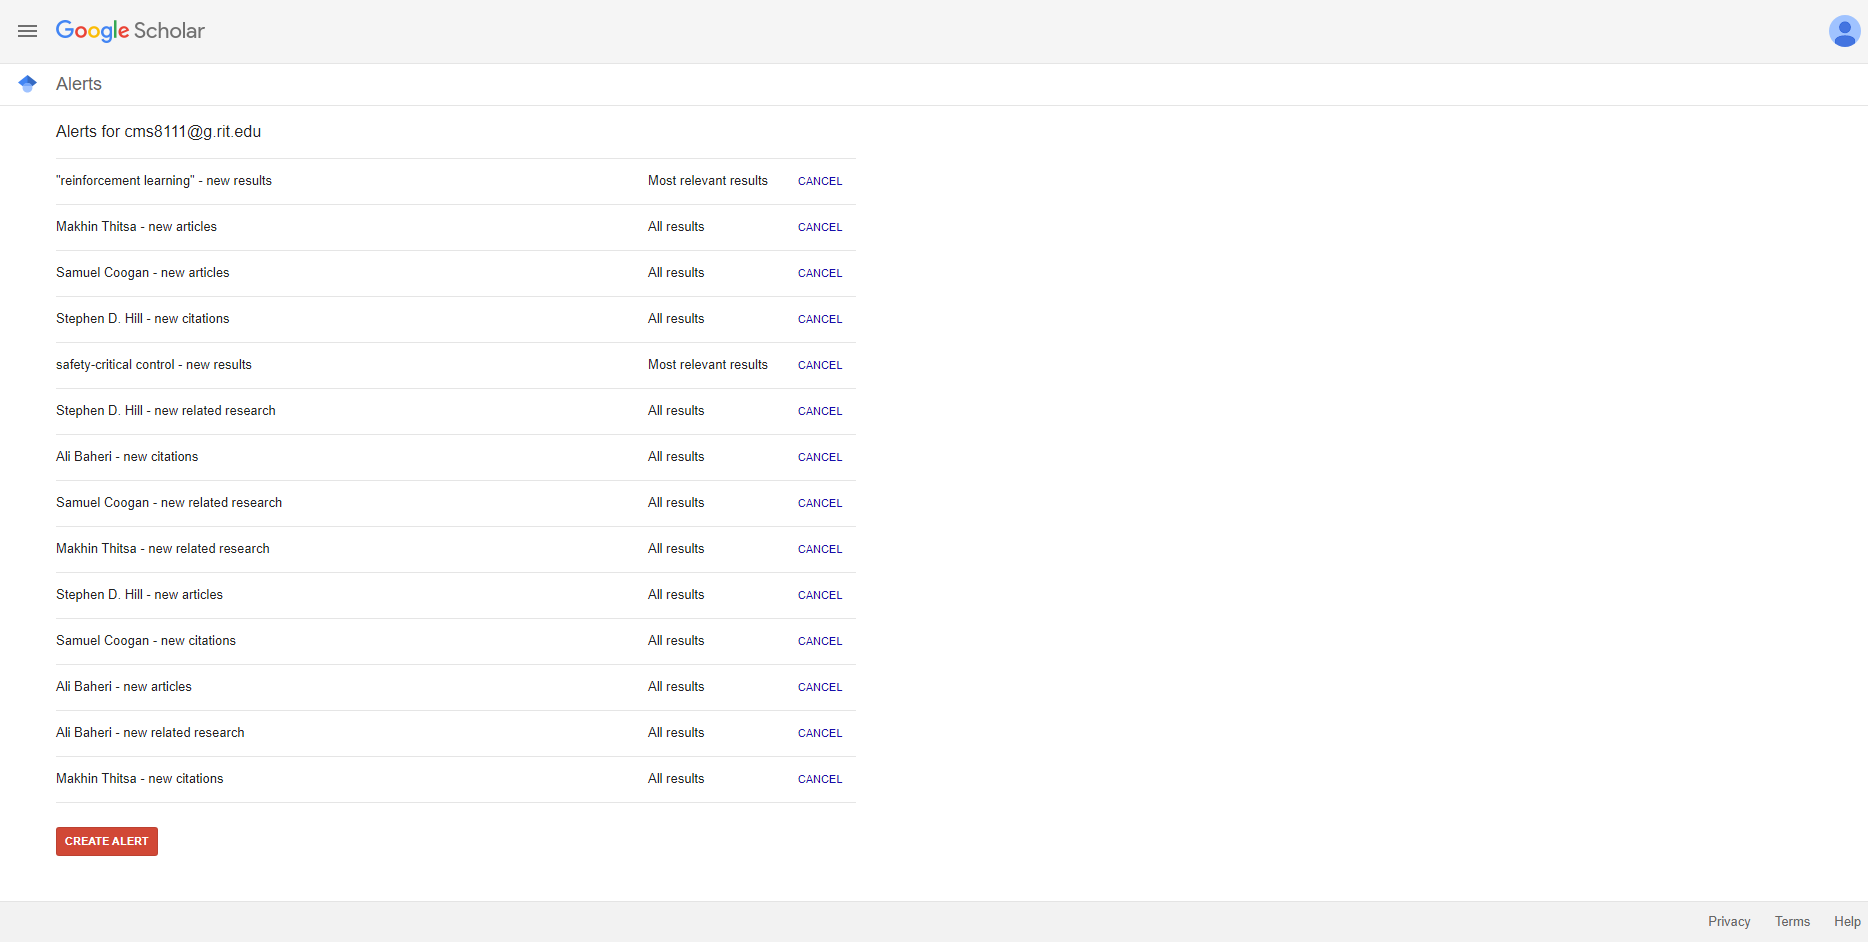
\includegraphics[width = \textwidth]{2024-09-19 18.20.07 scholar.google.com f39d6d4bc328.png}
        \caption{Screenshot of Google Scholar Alerts. Note that it includes both researchers and interesting keywords.}
        \label{fig:alerts}
        \end{figure}
    \end{problem}

    
\begin{problem}{$\#3$}
Here are three journals:
\begin{enumerate}
    \item IEEE Open Journal of Control Systems
    \item Automatica
    \item Journal of Machine Learning Research
\end{enumerate} 

See Table \ref{tab:journals} for more details.

\begin{table}[h!]
    \centering
    \caption{Journal information summary, with all details given. }
    \label{tab:journals}
    \resizebox{\textwidth}{!}{
    \begin{tabular}{@{}l l l l@{}}
    \toprule
    \textbf{Journal}                                 & \textbf{Publisher}                             & \textbf{Publication Frequency}              & \textbf{Average Review Time}                  \\ \midrule
    IEEE Open Journal of Control Systems             & IEEE                                          & Continuous, articles released individually  & $8$-$12$ weeks                               \\
    Automatica                                       & Elsevier                                      & Monthly, $28$ articles in recent issue      & $358$ days (ScienceDirect), typically $9$+ months \\
    Journal of Machine Learning Research (JMLR)      & JMLR, Inc. \& Microtome Publishing            & Continuous, $400$ articles in 2023 compendium & $3$-$6$ months                               \\ \bottomrule
    \end{tabular}
    }
    \end{table}

IEEE Open Journal of Control Systems is published by IEEE.  Publication of accepted papers on IEEE Xplore is guaranteed to be no more than 24 weeks after initial submission. This also means that articles are released individually rather than in batches.  Review times are generally on the order of $8$ to $12$ weeks, but this can vary. 

Automatica is published by Elsevier, with issues being monthly. The most current issue had $28$ articles published. Average review times seem long, with average submission to acceptance times being $358$ days according to ScienceDirect, but these may vary. Reviews have stated that time to publish is usually over $9$ months. 

Journal of Machine Learning Research (JMLR) is published by JMLR, Inc. and Microtome Publishing. Articles are published continuously upon acceptance, rather than in journal blocks, with average review time being about $3-6$ months. Volume $24$ (a compendium of all publications in the journal in $2023$) had $400$ entries. 
\end{problem}

\begin{problem}{$\#4$}

    Reinforcement learning and control strategies have converged in recent years, such as reinforcement learning based optimal control methods \cite{shi2025reinforcement} or in the emerging field of online non-stochastic control and decision making \cite{yan2023online}
    Engineered systems are designed to be safe, and so recent control theoretical work has focused on approaches to provide provable safety guarantees for critical, but high-dimensional systems, such as in Reinforcement Learning (RL).  Recently, methods using Hamilton-Jacobi (HL) reachability analysis have been proposed to provide provable safety guarantees for RL, by learning the HJ reachability value function while learning control policies \cite{ganai2024hamilton}.  Variations of Control Barrier Functions (CBFs) can also be used for ensuring the safety of learning-enabled systems, particularly for safe exploration for online RL \cite{cohen2023safe}. Interesting further developments could include implementing provable safety guarantees in policy-guided diffusion, a method to use diffusion models to generate trajectories and controllable synthetic training data \cite{jackson2024policy}. There is also promise in incorporating such work in RL paradigms with different notions of safety, such as welfare-centric fair reinforcement-learning, which casts fair learning as malfare-minimizing (non-maleficience) \cite{cousins2022fair}. 




\end{problem}

\begin{problem}{$\#5$}
Before I start designing my presentation, I should \textit{know my audience}. That is, I should see if it is meant to be for a conference, or a group meeting. or for a seminar. I should also be wary of \textit{time constraints}, including how much time I will need for questions and answers. Finally, before I start, I should decide on my goal and the main message I'd like to convey. 
\end{problem}
\newpage
\bibliography{ref}
\bibliographystyle{apacite}

\end{document}

